\section{Brevi Nozioni di Acustica}

In questa sezione saranno esposti, in maniera più o meno breve, i principi di
carattere fisico e percettivo che verranno utilizzati nell'implementazione
finale del riverbero atmosferico.

% Il campo della scienza che si occupa degli studi relativi alla fisica del suono
% si chiama \emph{acustica}, i cui primi passi sono stati mossi già dai primi \textit{pitagorici}
% portando innovazione ancora oggi. Di studi più recenti sulla percezione dell'evento sonoro
% da parte dell'uomo se ne occupa invece la \textit{psicoacustica}.

\subsection{Distanza dalla sorgente}

La distanza dalla sorgente sonora comporta una diminuzione di intensità. Dato
che l’onda si propaga in modo sferico, segue la legge dell’inverso del quadrato,
comportando una diminuzione di $6dB$ ad ogni raddoppio della distanza.

\subsection{Gas: temperatura e densità}

Parlare di temperatura è importante in quanto è un fattore che influisce in
diversi altri fattori presi in esame in questa tesi, ed è inoltre il punto di
partenza della mia ricerca. Dalla temperatura dipendono infatti la velocità del
suono nel mezzo e il valore di assorbimento atmosferico. La velocità del suono
possiamo calcolarla secondo la seguente formula:

\begin{equation}
C=\sqrt{\frac{\gamma Ps}{\rho}}
\end{equation}
dove

\begin{itemize}
      \item $\gamma$ è il coefficiente di dilatazione adiabatica
      \item $Ps$ è la pressione circostante
      \item $\rho$ è la densità del gas
\end{itemize}

La densità del gas, come per il coefficiente di dilatazione adiabatica, varia a
seconda della temperatura che, data la sua presenza in varie equazioni, diviene
un fattore determinante per la velocità del suono e dunque per le
caratteristiche del riverbero. Possiamo calcolare la densità tramite la seguente
formula% (pag 173):

\begin{equation}
\rho = \frac{stp*hg}{(1+t*0.00367)*hg}
\end{equation}

di cui:

\begin{itemize}
  \item $stp$ è la densità del gas a temperatura e pressione standard;
  \item $hg$ è la pressione barometrica del mercurio in centimetri;
  \item $t$ è la temperatura in gradi Celsius;
  \item $0.00367$ è il coefficiente di dilatazione termica,una costante comune
        a tutti i gas
\end{itemize}

Possiamo verificare la densità standard dei gas a tabella \ref{tab:dens}

\bigskip
\begin{table}[h]
\centering
\caption{Tabella raffigurante la densità di alcuni gas a \emph{}}
\label{tab:dens}
\begin{tabular}{lcr}
\toprule
Nome del gas & Simbolo & Densità($kg/m^2$) \\
\midrule
Aria & - & 1.2930 \\
Ammonia & $NH_3$ & 0.7710 \\
Nitrogen & $N_2$ & 1.2507 \\
Chlorine & $CI_2$ & 3.2170 \\
Carbon dioxide & $CO_2$ & 1.9760 \\
Hydrogen & $H_2$ & 0.0899 \\
Methane & $CH_4$ & 0.7170 \\
Carbon Monoxide & $CO$ & 1.2500 \\
Oxygen & $O$ &1.4290 \\
Water Vapour & $H_2O$ & 0.804 \\
\bottomrule
\end{tabular}
\end{table}
\smallskip

\subsection{Assorbimento atmosferico}

Rappresenta l’effetto di dissipazione dell’energia data dall’azione combinata
di viscosità e calore del mezzo. Perdite di energia aggiuntive sono dovute
all’umidità assoluta. Questo effetto comporta inoltre un aumento
dell’attenuazione con l’aumento delle frequenze.

\begin{figure}[h]
\centering
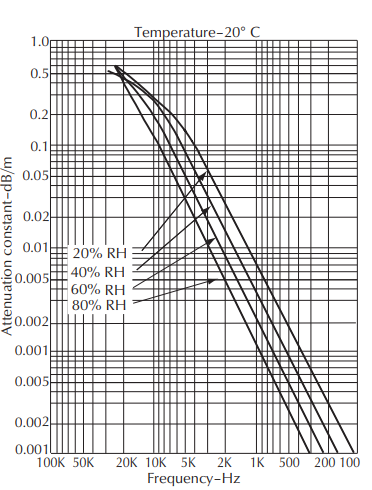
\includegraphics[width=%
0.50\textwidth]{assorbimento}
\caption{Tabella dei coefficenti di assorbimento dell'aria}
\label{fig:assorbimento}
\end{figure}

\subsection{Umidità}
Il livello di umidità del gas si riferisce alla presenza o meno di molecole
d’acqua nel mezzo. La sua influenza non è tanto impattante per quanto riguarda
la velocità dell’onda, ma sull’assorbimento acustico totale comportando un
abbattimento di intensità a diverse frequenze.

\subsection{Fenomeni di Riflessione}

Le riflessioni sono alla base di ciò che chiamiamo riverbero. Consistono nella
riflessione di un’onda sonora sulle diverse superfici che circondano l’evento
acustico, esse siano pareti oppure oggetti che si interpongono nella
propagazione dell’onda.

Affinché ci sia una riflessione, la superficie riflettente deve necessariamente
essere più larga di almeno $\frac{1}{4}$ della lunghezza d’onda. Quando
l’oggetto è più piccolo di questa soglia si ha una diffrazione, ovvero l’onda
sonora curva attorno ad esso.

Un altro fenomeno, che possiamo considerare inverso alla riflessione, è
\emph{l’assorbimento}. L’assorbimento è dovuto alle proprietà del materiale che,
appunto, al posto di riflettere l’onda assorbono parte dell’energia,
trattenendola e restituendo un’onda smorzata. Più un materiale è assorbente,
più sarà rapido il decadimento dell’energia sonora nello spazio fino a tornare
in una situazione di stabilità.

La condizione di stabilità sussiste infatti, quando la quantità di energia
assorbita è la medesima dell’energia prodotta.

\subsection{Fenomeni di Rifrazione}

La rifrazione similmente alla riflessione si ha quando è il mezzo di
trasmissione a subire delle variazioni, comportando dunque una differenza nella
propagazione in atto. Queste variazioni possono essere, per esempio,
temperatura, densità o direttamente un mezzo diverso, basti pensare ad un onda
prodotta in aria che incontra una superficie d’acqua.
